\newpage
\section{Distributed Database Concepts}

% Distributed Databases
\subsection{Distributed Databases}

I dati utilizzati nelle infrastrutture dei big data \hl{devono essere ACID}. Queste sistemi distribuiti sono \hl{composte da nodi che collaborano per compiere un task}. In queste infrastrutture andremo a distribuire le risorse sui nodi che cooperano in modo da avere \hl{ridondanza di dati}.

Esiste una \hl{relazione logica tra questi database connessi}, ma non tutti i nodi devono essere omogenei quindi possiamo al concetto di \hl{DISTRIBUTED DBMS} che deve gestire l'avere modelli dati connessi. 

Per quanto riguarda \hl{le query bisognera' riorganizzarle} per poter gestire i nodi distribuiti.


% Forme di trasparenza
\subsection{Forme di trasparenza}

Abbiamo varie forme di \hl{trasparenza rispetto all'utente}:

\begin{itemize}
    \item \hl{organizzazione dei dati}:

        \begin{itemize}
            \item local transparency
            \item naming transparency
        \end{itemize}
    
    \item \hl{ridondanza}: usata per ridurre la mancanza del servizio
    
    \item \hl{frammentazione dei dati}:

        \begin{itemize}
            \item \textbf{partizione orizzontale}: abbiamo una partizione delle tuple. La struttura dati è la stessa ma cambiano i dati salvati. Sarà completa se siamo in grado attraverso l’operazione di union di riavere la relazione iniziale completa
            
            \begin{figure}[H]
            \centering
            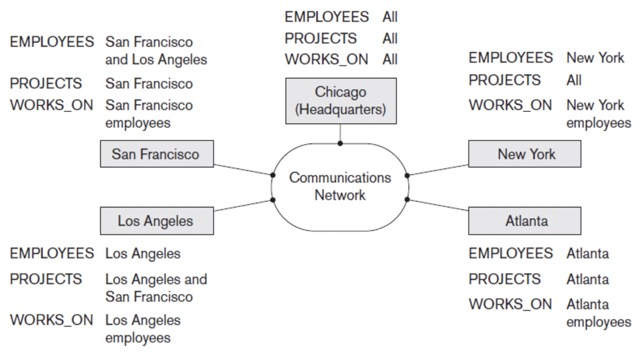
\includegraphics[scale=0.4]{partoriz.jpeg}
            \caption{Partizione orizzontale di un db} 
            \label{partoriz}
            \end{figure}

            \item \textbf{partizione verticale}: frammentazione del modello dati attraverso la partizione degli attributi che possono essere dislocati su più nodi
        \end{itemize}
    
\end{itemize}


% Affidabilità e disponibilità
\subsection{Affidabilità e disponibilità}

Per poter rispettare affidabilità e disponibilità usiamo la \hl{ridondanza}.

Eseguiamo una distribuzione dei dati \hl{per avere la possibilita' di scalare i dati in modo orizzontale o verticale} a seconda dell'uso che dobbiamo farne. Parliamo di:

\begin{itemize}
    \item \hl{horizzontal scalability}: poter \textbf{espandere il numero di nodi} del sistema
    \item \hl{vertical scalability}: poter espandere la \textbf{capacità di un singolo nodo}
    \item \hl{partition tolerance}: il sistema è \textbf{capace di operare anche se partizionato}
\end{itemize}


% Autonomia
\subsection{Autonomia}

La caratteristica principale della distribuzione è l'\hl{autonomia di ogni nodo rispetto agli altri}, quindi lo deve essere anche il loro contenuto, tenendo conto di:

\begin{itemize}
    \item \hl{design autonomy}: rappresenta indipendenza dei modelli dei dati e la \textbf{gestione delle transazioni tra i nodi}
    \item \hl{communication autonomy}: dà la possibilità di condividere le informazioni
    \item \hl{execution autonomy}: mi assicura che posso \textbf{eseguire una query}
\end{itemize}

Il \hl{vantaggio delle architetture distribuite} è una migliore facilità di sviluppo, disponibilità e performance.


% Frammenti
\subsection{Frammenti}

I frammenti sono le \hl{unita' logiche dei database} e possono essere:

\begin{itemize}
    \item \hl{frammentazione orizzontale}: divide le relazioni in orizzontale (\textbf{tuple})
    \item \hl{frammentazione verticale}: divide le relazioni in verticale (\textbf{colonne})
    \item \hl{frammentazione orizzontale completa}: se tramite \textbf{union} possiamo ricostruire la nostra lezione completamente
    \item \hl{frammentazione verticale completa}: usiamo la \textbf{join}
\end{itemize}

Spesso nella ricostruzione di un db possiamo trovare sia frammentazioni verticali che orizzontali, parliamo allora di \hl{frammentazione dello schema}.

Un DDBMS è in grado di gestire una frammentazione usando un \hl{ALLOCATION SCHEMA} che \hl{specifica come i frammenti del db sono distribuiti su quali nodi}.

Quando abbiamo dei dati possiamo avere la necessità di ridondanza. Questo non è il metodo migliore per chi si occupa di \hl{grandi moli di dati}, infatti bisognerà fare delle \hl{repliche a caldo che ogni tempo t} su un altro sito. In questi casi \hl{ci viene in soccorso il database journal} che \hl{tiene traccia dei log/modifiche} fatte al db, andando a prevenire eventuali errori dato che si potrà accedere ad una versione immediatamente precedente dei dati.

Potremo avere delle \hl{repliche totali o parziali}, replicando struttura e dati a secondo dello schema di replica presente del DDBMS.


% DDBMS
\subsection{DDBMS}

Potrebbero esserci dei problemi:

\begin{itemize}
    \item eccessive copie dei dati
    \item \hl{two phase commit}: dove un nodo quando ne aggiorna un altro ha la possibilità che fallisca e gli sia mandato un ACK -1, in questo casi bisognerà rincominciare tutto dall'inizio
\end{itemize}

Nella gestione delle ridondanza si utilizza un \hl{sito primario} che può essere sostituito, nel caso di malfunzionamenti, da uno secondario, andando a \hl{gestire le tabelle in modo parallelo}. Per capire chi sarà il nuovo responsabile del locking si usa un \hl{sistema a voto}. 

Quando noi \hl{eseguiamo una query in ambiente distribuito} possiamo usare il:

\begin{itemize}
    \item[] \hl{query mapping}: per capire \textbf{quali dati vengono utilizzati} dalla query e \textbf{dove si trovano} sui vari frammenti eseguendo quindi una \textbf{mappatura}. Successivamente \textbf{esegue la query in modo decentralizzato}
\end{itemize}

Da notare che il DDBMS permette l’\hl{ottimizzazione delle query}, indicano i valori più richiesti su un database. Per esempio l'utilizzo di indici sulle chiavi primarie ed ereditate per velocizzare il processo della query.


Per riuscire a \hl{ridurre la quantita' di dati che devo trasmettere}, usiamo un costrutto particolare: \hl{semi-join} che \hl{riduce il numero di tuple che trasmetto mandando soltanto la colonna di join} e prendendo unicamente i valori che mi vengono dalla join della tabella di partenza. 

Nei DDBMS relazionali sono usati i \hl{database federati} dove ho un \hl{modello dati condiviso} da tutti ma i \hl{singoli nodi dispongono di modelli dati indipendenti}, quindi ogni nodo mantiene uno schema generale che permette di comunicare con gli altri. Abbiamo \hl{3 dimesioni per il database distribuito}:

\begin{itemize}
    \item autonomia
    \item distribuzione
    \item eterogeneità
\end{itemize}


\begin{figure}[H]
\centering
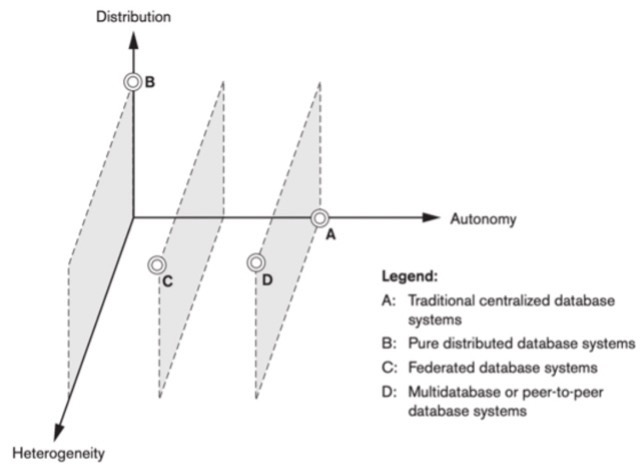
\includegraphics[scale=0.4]{dimddbms.jpeg}
\caption{Dimensioni del DDBMS} 
\label{dimddbms}
\end{figure}


